\chapter{Visualization}

\section{t-SNE visualization}
Embed high-dimensional points so that locally, pairwise distances are conserved i.e. similar things end up in similar places.
Dissimilar things end up wherever. Pronounced "tisni".

\begin{figure}[h]
  \centering
  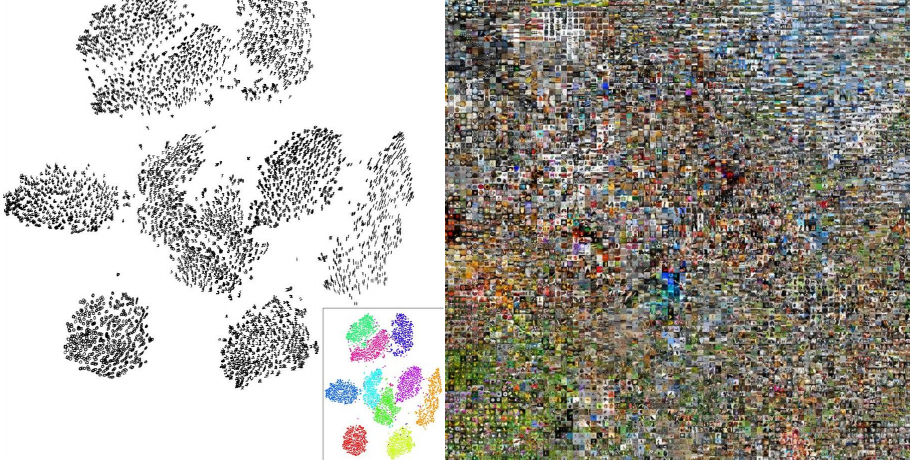
\includegraphics[width=0.6\textwidth]{Images/visualization/16.png}
  \caption{\textbf{Left}: Example embedding of MNIST digits (0-9) in 2D, \textbf{Right}: CIFAR-10 representation warped in a square shape}
\end{figure}

More CIFAR-10 examples \href{http://cs.stanford.edu/people/karpathy/cnnembed/}{here}

\section{Occlusions}
The idea is to create a hit map of the output probability of the CNN of the image in the left corresponding to the correct label as you slide an occlusion across the image.

This helps you understand what are the regions which contains the most valuable features, for the CNN, in the image.

For example, in the first row, we can observe that the probability of the left image being a Pomeranian decreases when we cover its face.

\begin{figure}[h]
  \centering
  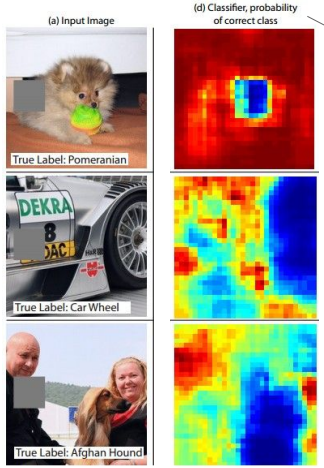
\includegraphics[width=0.25\textwidth]{Images/visualization/3.png}
  \caption{Visualize with occlusions}
\end{figure}


\section{Visualizing Activations}
How can we compute the gradient of any arbitrary neuron in the network w.r.t. the image?

\begin{figure}[h]
  \centering
  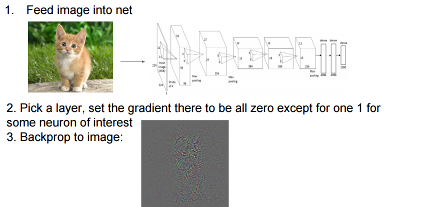
\includegraphics[width=0.6\textwidth]{Images/visualization/4.png}
  \caption{Visualize with occlusions}
\end{figure}

The output image gradients is not that good to understand what is going on. We will now see two strategies to obtain "better looking" gradients: Deconv approaches and

\section{Deconv approaches}

We are trying to see what parts of the input image are exciting a specific neuron. The idea to get a better looking gradient image is only to take into account the positive gradients. In this way we remove the noise caused by mixing positive and negative gradients.

The ReLU layer only backprop the gradient of the activations that where positive at the forward pass.

With Deconv, we must hack this behavior and change it so the ReLU layers only backprop positive gradients and do not care if the forward activations where positive or negative.

\begin{figure}[h]
  \centering
  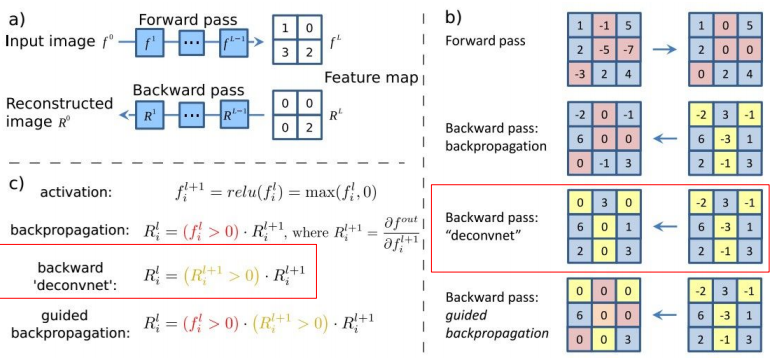
\includegraphics[width=0.8\textwidth]{Images/visualization/5.png}
  \caption{Deconv approaches}
\end{figure}

Now we can show what excites a specific neuron. The figures below show a grid of neurons at each layer. For each neuron we can see the image that arrived to that neuron and what parts of this image excited the neuron. So the deeper the neuron the bigger the area of the original image it observes. Also, it can be seen that the deeper the neuron the higher feature representation.

\begin{figure}[h]
  \centering
  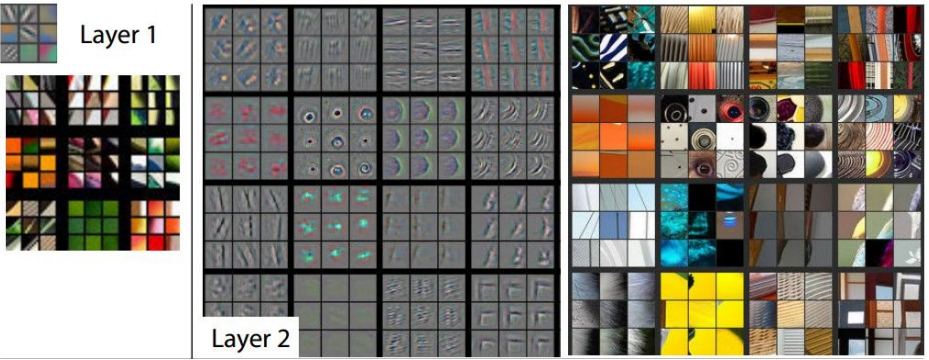
\includegraphics[width=0.8\textwidth]{Images/visualization/6.png}
  \caption{Deconv approaches layers 1 and 2}
\end{figure}

\begin{figure}[h]
  \centering
  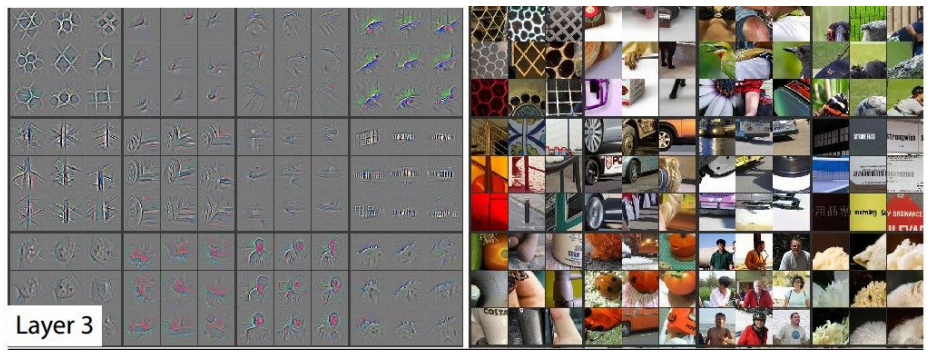
\includegraphics[width=0.8\textwidth]{Images/visualization/7.png}
  \caption{Deconv approaches layer 3}
\end{figure}

\begin{figure}[h]
  \centering
  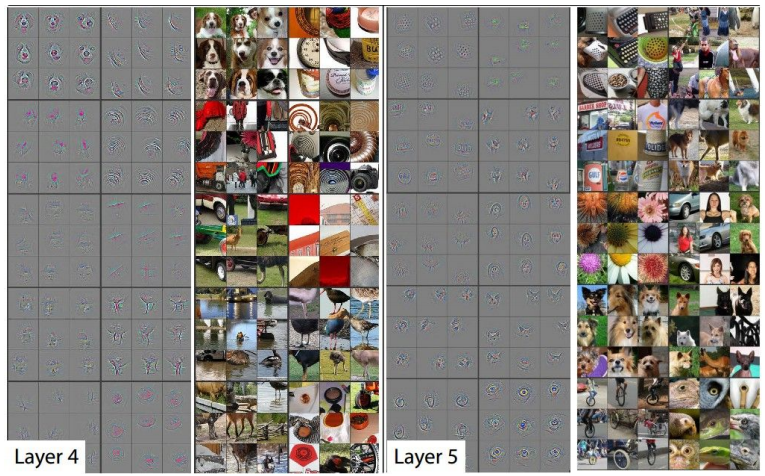
\includegraphics[width=0.8\textwidth]{Images/visualization/8.png}
  \caption{Deconv approaches layers 4 and 5}
\end{figure}


\section{Optimization to image}
How can we find an image that maximizes some class score?
\begin{figure}[h]
  \centering
  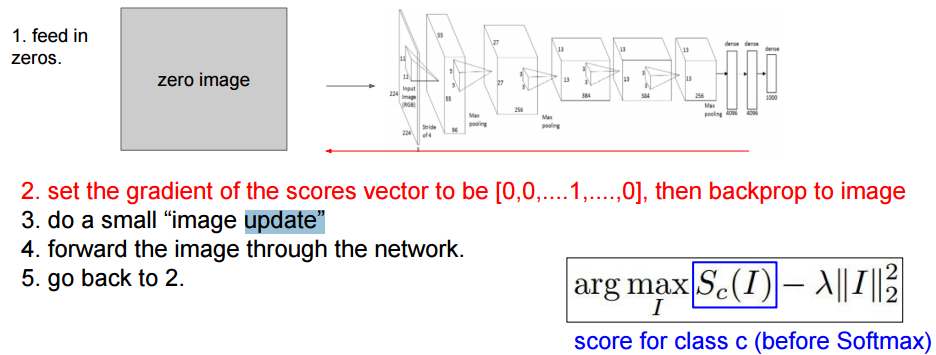
\includegraphics[width=0.6\textwidth]{Images/visualization/9.png}
  \caption{Optimize an image to maximize the score of a specific class}
\end{figure}

\begin{figure}[h]
  \centering
  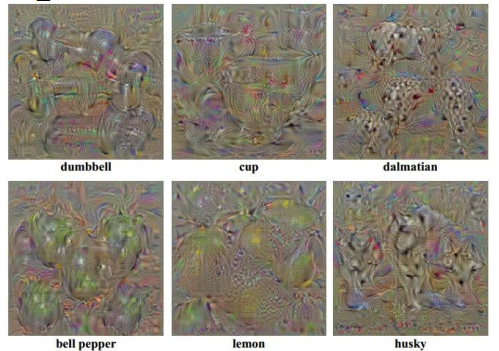
\includegraphics[width=0.45\textwidth]{Images/visualization/10.png}
  \caption{Optimize an image to maximize the score of a specific class output}
\end{figure}


\section{Visualizing Data Gradients}
\begin{enumerate}
\item Feed an input image
\item Set the gradient of the scores vector be [0,0,..,0,1,0,...0] where 1 is the ground-truth label class of the image
\item Backprop to the image
\item For each pixel of the image store the max gradient value across all the channels
\item Plot the gradients
\end{enumerate}

\begin{figure}[h]
  \centering
  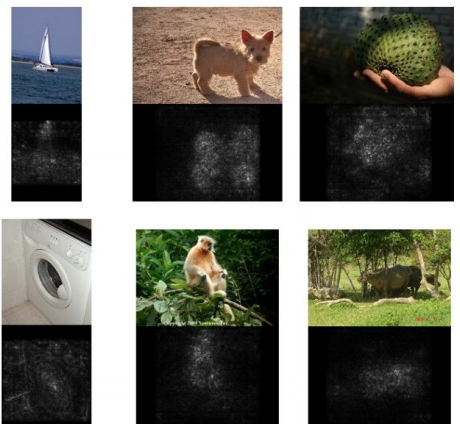
\includegraphics[width=0.3\textwidth]{Images/visualization/11.png}
  \caption{Data gradients output}
\end{figure}


The interpretation of the results are that the staff that is black is not influencing the score of the image. So you can wiggle them and the score will not change. So at the end it is telling you the are of the image that is influencing the network.

\section{DeepDream}

\begin{figure}[h]
  \centering
  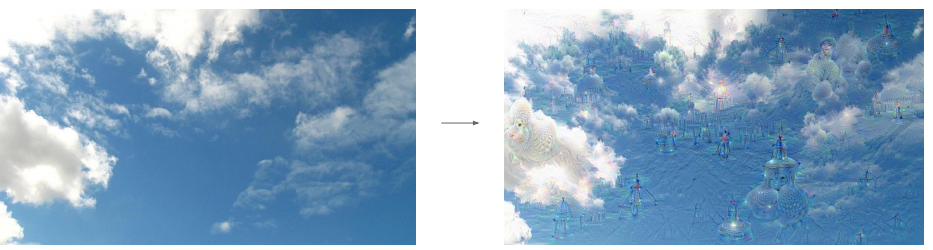
\includegraphics[width=0.6\textwidth]{Images/visualization/13.png}
  \caption{DeepDream output}
\end{figure}

DeepDream \href{http://cs.stanford.edu/people/karpathy/cnnembed/}{link} 

It normally hallucinate a lot of dogs because there are a lot of dog samples in ImageNet (because there are a lot of different dog classes).

\begin{figure}[h]
  \centering
  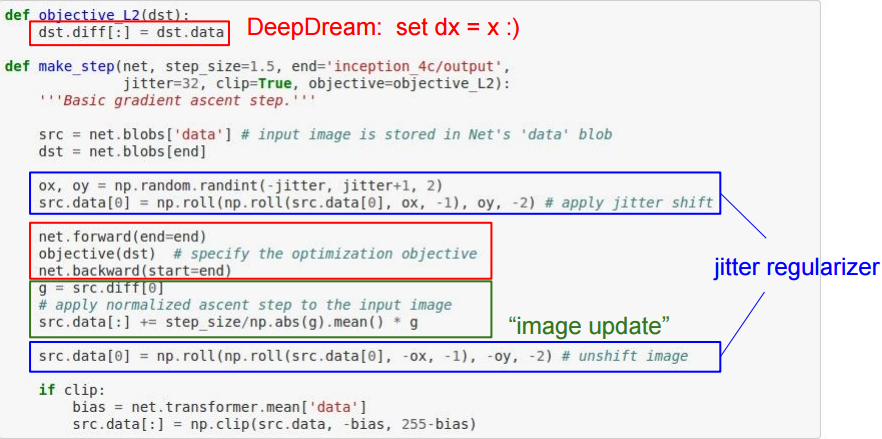
\includegraphics[width=0.8\textwidth]{Images/visualization/12.png}
  \caption{DeepDream code}
\end{figure}

At the end, the only thing DeepDream is doing is: given a layer immediately after a ReLU layer, it sets the gradients equal to the activation values. So if you iteratively update the image with the gradients, you are modifying the image to increase whatever it is exiting the selected layer.

In other words, DeepDream modifies the image in a way that ``boosts” all activations. This creates a feedback loop: e.g. any slightly detected dog face will be made more and more dog like over time.

\section{DeepArt}
Explained at cs231n lecture 9

\section{Adversarial data - Fooling networks}
It is very simple to fool a CNN. Images are super high dimensional objects (one dimension for each pixel). The training images are constrained to a small manifold and we are training ConvNets over it. The trained ConvNet works extremely well inside that manifold, but outside of it is complete random.

\begin{figure}[h]
  \centering
  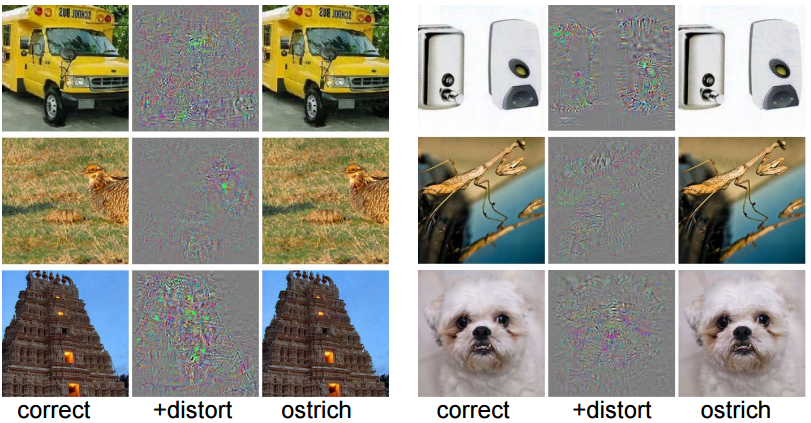
\includegraphics[width=0.65\textwidth]{Images/visualization/14.png}
  \caption{Adversarial data examples}
\end{figure}

The think is that during the forward pass we are applying dot product over all the dimensions of the data (one per pixel) so if we change the input a tiny bit but all in the correct way, the dot product output is going to change a lot.

\begin{figure}[h]
  \centering
  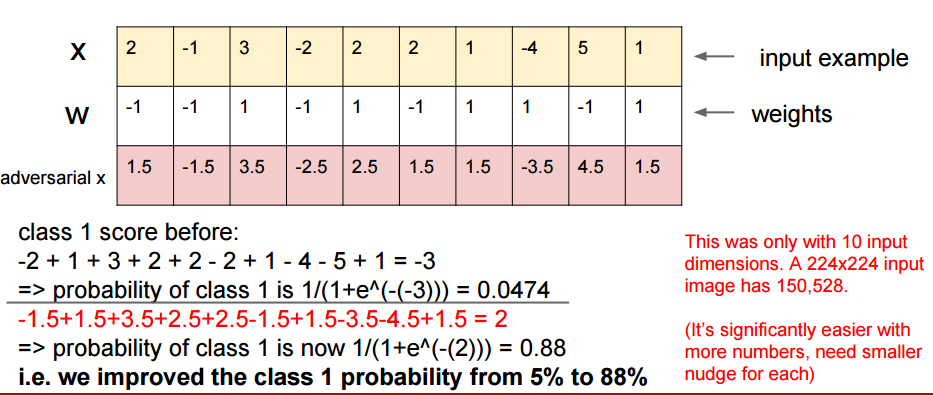
\includegraphics[width=0.8\textwidth]{Images/visualization/15.png}
  \caption{Adversarial data case example}
\end{figure}

This is not a problem of deep learning, its is a problem in learning in general. There are some ways of decreasing this effect. One is to train also with adversarial examples; it will be more robust to them but the classifier accuracy will decrease. Another one is to instead of classifying the hole image, classify chunks.